\chapter{分离变量法}

这是一种先假设解可以分离变量为\(u(x,t)=X(x)T(t)\),根据定解条件得到一个关于空间\(x\)的常微分方程和一个关于时间的\(t\)的常微分方程,求解\(X(x),T(t)\),最后说明这个解是存在,唯一,且稳定的求解方法。这里并没有很充分的理由说明为什么可以分离变量,但是它得到的结果是正确的。

为排版方便,部分公式中的内容(常见于三角函数中)进行了以下替换:\[w=\frac{n\pi a}{l}\]%属实是难倒我了

\section{预备知识}

\subsection{函数内积}

在区间\([a,b]\)上定义二个函数\(f_1(x)\)和\(f_2(x)\),则它们的内积定义为:
\[
\langle f_1,f_2\rangle=\int_{a}^{b}{f_1(x)f_2(x)\,\mathrm{d}x}
\]

\subsection{正交函数}

二个函数\(f_1(x)\)和\(f_2(x)\)在区间\([a,b]\)上是正交的,则它们的内积为0,即\(\langle f_1,f_2\rangle=\int_{a}^{b}{f_1(x)f_2(x)\,\mathrm{d}x}=0\)

例如:\(f(x)=x^2,f(x)=x^3\)在\([-1,1]\)上是正交的。

\subsection{正交函数系}

设有一族\([a,b]\)上的函数,满足\(\int_{a}^{b}{\varphi_m(x)\varphi_n(x)\,\mathrm{d}x}\begin{cases}=0&m\neq n\\\neq0&m=n\end{cases}m,n=0,1,\ldots\)

则称该函数系为定义域上的正交函数系,简称正交系,记为\(\{\varphi_n\}_{n=0}^\infty\)或\(\{\varphi_n\}\)

重要性质:线性无关。例如:函数系\(1,\cos{\frac{\pi x}{l}},\sin{\frac{\pi x}{l}},\ldots,\cos{\frac{wx}{a}},\sin{\frac{wx}{a}},\ldots\)为\([-l,l]\)上的正交函数系。

\subsection{范数}

一个函数\(f(x)\),若积分\(\int_{a}^{b}{f^2(x)\,\mathrm{d}x}\)存在,则称\(f\)平方可积

将\(\|\varphi\|^2=\left[\int_a^b\varphi^2(x)\,\mathrm{d}x\right]^{\frac{1}{2}}\)称为\(\varphi\)在\(L^2([a,b])\)中的范数。范数便是函数的度量。

\subsection{正交函数集的标准化}

假设有正交函数系:\(1,\cos{\frac{\pi x}{l}},\sin{\frac{\pi x}{l}},\ldots,\cos{\frac{wx}{a}},\sin{\frac{wx}{a}},\ldots\)为\([-l,l]\)上的正交函数系

令\(l=\pi\),然后\(\frac{(\ )}{\sqrt{\int_{-\pi}^{\pi}{(\ )^2\,\mathrm{d}x}}}\),可得\(\frac{1}{\sqrt{2\pi}},\frac{\cos{x}}{\sqrt\pi},\frac{\sin{x}}{\sqrt\pi},\ldots,\frac{\cos{nx}}{\sqrt\pi},\frac{\sin{nx}}{\sqrt\pi},\ldots\)为上的\([-\pi,\pi]\)标准正交系。正交系的一个重要性质就是线性无关,两两正交。

\subsection{函数的傅里叶级数展开}

设\(f(x)\)是\(2l\)为周期的函数,在\([-l,l]\)上满足以下条件:
\begin{enumerate}
    \item 连续或只有有限个第一类间断点
    \item 至多有有限个极值点
\end{enumerate}
\[
f(x)\sim\frac{a_0}{2}+\sum_{n=1}^{\infty}{\left(a_n\cos\frac{wx}{a}+b_n\sin\frac{wx}{a}\right)}
\]

其中\(\begin{cases}a_n=\frac{1}{l}\int_{-l}^lf(x)\cos\frac{wx}{a}\,\mathrm{d}x,n=0,1,\ldots\\b_n=\frac{1}{l}\int_{-l}^lf(x)\sin\frac{wx}{a}\,\mathrm{d}x,n=1,2,\ldots\end{cases}\)且当\(x\)是\(f(x)\)连续点时,级数收敛于\(f(x)\)(或\(\frac{1}{2}[f(x^-)+f(x^+)]\)不连续时)
\subsection{二阶线性齐次常微分方程的求解问题}

\subsubsection{问题}
\[
y''+py'+qy=0
\]

令\(y(x)=\mathrm{e}^{rx}\),有\(r^2+pr+q=0\),两个根为\(r_1,r_2\)

\subsubsection{通解}
\begin{enumerate}
    \item 相异实根:\(y=C_1\mathrm{e}^{r_1x}+C_2\mathrm{e}^{r_2x}\)
    \item 相等实根:\(y=\left(C_1+C_2x\right)\mathrm{e}^{r}x\)根据参数变异法所求
    \item 共轭复根:\(\alpha\pm w\mathrm{i},y=\mathrm{e}^{\mathbf{\alpha}x}[C_1\cos( wx)+C_2\sin( wx)]\)
\end{enumerate}

\section{波动方程初边值问题分离变量法求解}

\subsection{Fourier方法}

\paragraph{条件}物理上,机械振动或电磁振动可以看成是多个简谐振动(驻波)\(\mathrm{e}^{\mathrm{i}w(t+cx)}=\mathrm{e}^{\mathrm{i}wt}\mathrm{e}^{\mathrm{i}kt}\)其中\(k=cw\)的叠加。数学上,驻波是只含变量\(x\)的函数与只含\(t\)的函数的乘积,即具有变量分离的形式。

\paragraph{求解}由此受到启发,求解线性方程定解问题时,可尝试先求出齐次方程和齐次边界条件的具有变量分离形式的解,\(u_n(x,t)=X_n(x)T_n(t),n=1,2,\cdots\),然后把它们叠加起来,即\(u(x,t)=\sum\limits_{n=1}^{\infty} C_nX_n(x)T_n(t)\),最后利用初始条件确定各项中的系数,使其成为定解问题的解。

\subsubsection{分离变量法求解波动方程定解问题}

\paragraph{问题}
\[\begin{cases}
u_{tt}=a^2u_{xx},0<x<l,t>0\\
u(x,0)=\varphi(x),u_t(x,0)=\psi(x)\\
u(0,t)=u(l,t)=0\quad\text{两端固定}
\end{cases}\]

\paragraph{分离变量}设问题有非零(非平凡)的变量分离解\(u(x,t)=X(x)T(t)\),将它回代到原式中,由\(u_{tt}=a^2u_{xx}\)得:
\[
X(x)T''(t)=a^2X''(x)T(t)
\]

变量整理\(\frac{T''(t)}{a^T(t)}=\frac{X''(x)}{X(x)}=-\lambda\),得:
\[\begin{cases}
X''(x)+\lambda X(x)=0,0<x<l\\
T''(t)+\lambda a^2T(t)=0,t>0
\end{cases}\]

其边界由\(u(0,t)=u(l,t)=0\Rightarrow x(0)T(t)=X(l)T(t)=0\)得:\(X(0)=X(l)=0\)

\paragraph{特征值问题}
\[\begin{cases}
X''(x)+\lambda X(x)=0,0<x<l\\X(0)=X(l)=0
\end{cases}\]
\begin{enumerate}
    \item 当\(\lambda<0\)时\(X(x)=C_1\mathrm{e}^{\sqrt{-\lambda}x}+C_2\mathrm{e}^{-\sqrt{-\lambda}x},X(0)=x(l)=0\),解得\(C_1=C_2=0\)不符合非零解的要求,因此,\(\lambda<0\)不是特征值
    \item 当\(\lambda=0\)时\(X(x)=C_1x+C_2,X(0)=X(l)=0\)解得:\(X(x)\equiv0\)因此,\(\lambda=0\)不是特征值
    \item 当\(\lambda>0\)时\[X(x)=C_1\cos{\sqrt\lambda x}+C_2\sin{\sqrt\lambda x},X(0)=0\]
    解得:\(C_1=0\)所以:
    \[X(x)=C_2\sin{\sqrt\lambda x}\]
    又:\(X(l)=0\)所以:
    \[C_2\sin{(\sqrt\lambda l)}=0\]
    解得:\(\sqrt\lambda l=n\pi\)由于:\(\lambda=a^2>0\)最后得到
    \[\lambda=\left(\frac{n\pi}{l}\right)^2,X(x)=C_2\sin\frac{wx}{a}\]
    其中\(n=1,2,\ldots\),这里\(C_2\)可视为1,加下表\(n\)是因为这个有多个特解,用下表加以区分,当\(X_n(x)\)和\(T_n(t)\)都求出来后,得到\(u_n(x,t)\)。最后利用叠加原理,将\(u\)的\(n\)个解叠加在一起,使其满足条件,得到通解\(u(x,t)\)。
\end{enumerate}

\paragraph{其他方程}求解\(T(t)\)常微分方程,,注意\(\lambda=\lambda_n=\left(\frac{n\pi}{l}\right)^2\)
\[
T_n(t)=A_n\cos{w t}+B_n\sin{w t}
\]

得到特解\(u_n(x,t)\)其中\(a_n=C_2A_n,b_n=C_2B_n\)
\[
u_n(x,t)=\left(a_n\cos{w t}+b_n\sin{w t}\right)\sin\frac{wx}{a},n=1,2,3,\ldots
\]


\paragraph{特解叠加}
\[
u(x,t)=\sum_{n=1}^{\infty}{u_n(x,t)}=\sum_{n=1}^{\infty}{\left(a_n\cos w t+b_n\sin w t\right)\sin\frac{wx}{a}}
\]

将\(n\)从结果中去除,且要确保该级数收敛于\(u(x,t)\),结果与\(n\)无关。

\paragraph{系数确定}

确定\(a_n,b_n\)的值。利用初始条件\(u(x,0)=\phi(x),u_t(x,0)=\psi(x)\),得到:
\[\begin{cases}
\phi(x)=u(x,0)=\sum\limits_{n=1}^{+\infty}a_n\sin\frac{wx}{a}\\
\psi(x)=u_t(x,o)=\sum\limits_{n=1}^{+\infty}b_n\frac{n\pi a}{l}\sin\frac{wx}{a}
\end{cases}\]

傅里叶正弦级数展开:
\[\begin{cases}
a_n=\frac{2}{l}\int_0^l\phi(x)\sin\frac{wx}{a}\,\mathrm{d}x\\
b_n=\frac{2}{n\pi a}\int_0^l\phi(x)\sin\frac{wx}{a}\,\mathrm{d}x
\end{cases}\]

其中\(n=1,2,\ldots\)

\subsubsection{解的物理意义}

\paragraph{驻波}
\begin{align*}
u(x,t)=&\sum_{n=1}^{\infty}{u_n(x,t)}=u_1(x,t)+u_2(x,t)+u_3(x,t)+\cdots\\
u_n(x,t)=&\left(a_n\cos{\frac{n\pi a}{l}t}+b_n\sin{\frac{n\pi a}{l}t}\right)\sin{\left(\frac{n\pi}{l}x\right)}\\
=&\sqrt{a_n^2+b_n^2}\cos\left(\frac{n\pi a}{l}t+\alpha_n\right)\sin\left(\frac{n\pi}{l}x\right)\\
=&N_n\cos{( w_nt+\alpha_n)}\sin\left(\frac{n\pi}{l}x\right)
\end{align*}

其中:强度/振幅\(N_n=\sqrt{a_n^2+b_n^2}\),圆频率\( w_n\frac{n\pi a}{l}\),初相\(\sin a_n=-\frac{b_n}{N_n},\cos a_n=\frac{a_n}{N_n}\)

\begin{figure}[htbp]
    \centering
    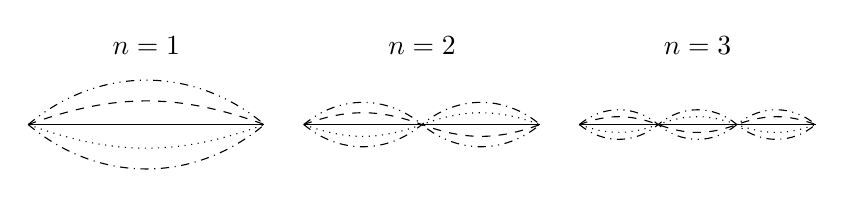
\begin{tikzpicture}[>=latex]
    \foreach \n/\l in {-40/dash dot,-20/dotted,0/,20/dashed,40/dash dot dot}{
    \draw[\l] (0,0)to[bend left=\n](3,0) (3.5,0)to[bend left=\n](5,0)to[bend right=\n](6.5,0) (7,0)to[bend left=\n](8,0)to[bend right=\n](9,0)to[bend left=\n](10,0);
    }
    \foreach \x in {1,2,3}{
    \node at(3.5*\x-2,1){\(n=\x\)};
    }
    \end{tikzpicture}
    \caption{驻波}\label{pic:stop}
\end{figure}

\paragraph{基频}\(\frac{\pi a}{l}\)最低频率,其他频率是它的整数倍。解的级数可以看作一系列频率成倍增长,相位不同,振幅不同的驻波的线性叠加而成。因此分离变量法也叫做驻波法。

\subsection{自由边界条件下波动方程问题的求解}

\paragraph{问题}\(\begin{cases}
u_{tt}=a^2u_{xx},0<x<l,t>0\\
u(x,0)=\phi(x),u_t(x)=\psi(x)\\
u_x(0,t)=u_x(l,t)=0
\end{cases}\)

\paragraph{分离变量}设问题有非零(非平凡)的变量分离解\(u(x,t)=X(x)T(t)\)

\paragraph{特征值问题}\(\begin{cases}X''(x)+\lambda X(x)=0,0<x<l\\
T''(t)+\lambda a^2T(t)=0,t>0\\
X'(0)=X'(l)=0\end{cases}\)

\paragraph{特解}\(u_n(x,t)=T_n(t)X_n(x)=\begin{cases}
(C_0+D_0t)A_0,n=0\\
(C_n\cos\frac{n\pi at}{l}+D_n\sin\frac{n\pi at}{l})A_n\cos\frac{n\pi x}{l},n=1,2,\ldots
\end{cases}\)

\paragraph{通解}\(u(x,t)=a_0+b_0t+\sum\limits_{n=1}^{\infty}{\left(a_n\cos{w t}+b_n\sin{w t}\right)\cos{\frac{wx}{a}}}\)

\paragraph{系数确定}确定\(a_n,b_n\)的值。利用初始条件\(u(x,0)=\phi(x),u_t(x,0)=\psi(x)\)和特征函数的正交性得到:
\[
\begin{cases}
a_n=\frac{1}{l}\int_0^l\phi(x)\,\mathrm{d}x\\
b_n=\frac{1}{l}\int_0^l\phi(x)\,\mathrm{d}x
\end{cases}\quad
\begin{cases}
a_n=\frac{2}{l}\int_0^l\phi(x)\sin\frac{wx}{a}\,\mathrm{d}x,n=1,2,\ldots\\
b_n=\frac{2}{n\pi a}\int_0^l\phi(x)\sin\frac{wx}{a}\,\mathrm{d}x,n=1,2,\ldots
\end{cases}
\]

\section{非齐次问题的求解}

\subsection{非齐次方程+齐次边界条件}

\paragraph{问题}\(\begin{cases}u_{tt}=a^2u_{xx}+f(x,t),0<x<l,t>0\\u(x,0)=\phi(x),u_t(x,0)=\psi(x)\\u(0,t)=u(l,t)=0\end{cases}\)

\paragraph{引例*}求解\(Ax=b,A_{n\times n}\)
\begin{enumerate}
	\item \(Ax=\lambda x\Rightarrow\begin{matrix}\lambda_1&\ldots&\lambda_n\\k_1&\ldots&k_n\\\end{matrix}\)满足\(Ak_i=\lambda k_i\)这些特征值对应的特征向量两两正交。
	\item 将\(x,b\)写为\(k_i\)的线性组合形式(例如\(x=\alpha_1k_1+\alpha_2k_2+\cdots+\alpha_nk_n,b=\langle b,k_1\rangle+\langle b,k_2\rangle+\cdots+\langle b,k_n\rangle\))
	\item 将它们代入\(Ax=b\),得\(\alpha_1\lambda_1k_1+\alpha_2\lambda_2k_2+\ldots+\alpha_n\lambda_nk_n=\langle b,k_1\rangle k_1+\langle b,k_2\rangle k_2+\cdots+\langle b,k_n\rangle k_n\)
	\item 比对系数相同:\(\alpha_i=\frac{\langle b,k_i\rangle}{\lambda_i}\)
\end{enumerate}

\paragraph{第一步}求正交基(特征函数系)

设问题有非零(非平凡)的变量分离解\(u(x,t)=X(x)T(t)\)则代入齐次问题有
\[\begin{cases}
X''(x)+\lambda X(x)=0\\
X(0)=X(l)=0
\end{cases}\]

由此解得特征函数为:
\[
X_n(x)=C_n\sin{\frac{n\pi x}{t}},n=1,2,\ldots
\]

\paragraph{第二步}把定解问题中的未知函数和已知函数写成特征函数展开的形式
\[
u(x,t)=\sum_{n=1}^{\infty}{T_n(t)\sin{\frac{wx}{a}}}
\]

\(T_n(t)\)为待定系数\(f(x,t)=\sum\limits_{n=1}^{\infty}{f_n(t)\sin{\frac{wx}{a}}}\)

每个方向的投影系数:
\[
f_n(t)=\frac{\left(f(x,t),\sin{\frac{wx}{a}}\right)}{\left(\sin{\frac{wx}{a}},\sin{\frac{wx}{a}}\right)}\longrightarrow f_n(t)=\frac{2}{l}\int_{0}^{l} f(x,t)\sin{\frac{wx}{a}\,\mathrm{d}x}
\]

初始条件:
\[
\phi(x)=u(x,0)=\sum_{n=1}^{\infty} T_n(0)\sin{\frac{wx}{a}},\psi(x)=u_t(x,0)=\sum_{n=1}^{\infty} T_n'(0)\sin{\frac{wx}{a}}
\]

\paragraph{第三步}关于\(T_n(t)\)的定解问题:将上述函数的级数展开形式代入原方程,求展开系数:
\[
\sum_{n=1}^{\infty}{\left[T_n''(t)+w^2\left(\frac{n\pi}{l}\right)^2T_n(t)\right]\sin{\frac{wx}{a}}}=\sum_{n=1}^{\infty}{f_n(t)\sin{\frac{wx}{a}}}
\]

该方程通解为其齐次方程的通解+其自身的一个特解
\[\begin{cases}
T_n''(t)+\left(\frac{n\pi a}{l}\right)^2T_n(t)=f_n(t)\\T_n(0)=\frac{2}{l}\int_{0}^{l}\phi(x)\sin{\frac{wx}{a}\,\mathrm{d}x}:=a_n\\T_n'(0)=\frac{2}{l}\int_{0}^{l}\psi(x)\sin{\frac{wx}{a}\,\mathrm{d}x}:=b_n
\end{cases}\]

\paragraph{第四步}用参数变易法解关于\(T_n(t)\)的定解问题
\begin{enumerate}
	\item 范定方程:\(T_n'\mathrm{e}(t)+\left(\frac{n\pi a}{l}\right)^2T_n(t)=0\)
	\item 通解:\(T_n(t)=C_1\cos w t+C_2\sin w t\)
	\item 参数变易:\(T_n(t)=C_1(t)\cos w t+C_2(t)\sin w t\)
\end{enumerate}

\paragraph{第五步}确定系数\(C_1(t),C_2(t)\),求解\(T_n''(t)+\left(\frac{n\pi a}{l}\right)^2T_n(t)=f_n(t)\)的一个特解。

两边求导:
\[
T'(t)=C_1'(t)\cos w t-w C_1(t)\sin w t+C_2'(t)\sin w t+ w C_2(t)\cos w t
\]

为简化方程,令\(C_1'(t)\cos w t+C_2'(t)\sin w t=0\)则有:
\[
T_n''(t)=-w C_1'(t)\sin w t-w^2C_1(t)\cos{w t}+ w C_2'(t)\cos{w t}-w^2C_2(t)\sin{w t}
\]

回代方程:\(T_n''(t)+ w^2T_n(t)=f_n(t)\)得:
\[
-C_1'(t)\sin{w t}+C_2'(t)\cos{w t}=\frac{1}{w}f_n(t)
\]

可使用克莱姆法则求解\(C_1'(t),C_2'(t)\)
\begin{gather*}
C_1'(t)=-\frac{1}{w}\int_{0}^{t}\sin{\frac{n\pi a\tau}{l}f_n\tau}\,\mathrm{d}\tau\\
C_2'(t)=\frac{1}{w}\int_{0}^{t}\cos{\frac{n\pi a\tau}{l}f_n\tau}\,\mathrm{d}\tau
\end{gather*}

\paragraph{第六步}确定\(T_n(t)\)
方程\(T_n''(t)+\left( w\right)^2T_n(t)=0\)

解:
\[
T_n(t)=C_1\cos{w t}+C_2\sin{w t}+C_1(t)\cos{w t}+C_2(t)\sin{w t}
\]

其中\(\begin{cases}C_1(t)=-\frac{1}{w}\int_{0}^{t}\sin{\frac{n\pi a\tau}{l}f_n(\tau)}\,\mathrm{d}\tau\\C_2(t)=\frac{1}{w}\int_{0}^{t}\cos{\frac{n\pi a\tau}{l}f_n(\tau)}\,\mathrm{d}\tau\end{cases}\)代入方程并化简可得通解表达:
\[
T_n(t)=C_1\cos{w t}+C_2\sin{w t}+\frac{1}{w}\int_{0}^{t}{f_n(\tau)\sin{w(t-\tau)\,\mathrm{d}\tau}}
\]

边界代入又有:
\[\begin{cases}
T_n(0)=\frac{2}{l}\int_{0}^{l}\phi(x)\sin{\frac{wx}{a}\,\mathrm{d}x}:=a_n\\T_n'(0)=\frac{2}{l}\int_{0}^{l}\psi(x)\sin{\frac{wx}{a}\,\mathrm{d}x}:=b_n
\end{cases}\]

故:\(T_n(0)=C_1=a_n,T_n'(0)=C_2=\frac{1}{w}b_n\)最终得到:
\[
T_n(t)=a_n\cos{w t}+\frac{{lb}_n}{n\pi a}\sin{w t}+\frac{1}{w}\int_{o}^{t}{f_n(\tau)\sin{w(t-\tau)}\,\mathrm{d}\tau}
\]

\paragraph{第七步}给出原问题的解
\[
u(x,t)=\sum_{n=1}^{\infty}{\left(a_n\cos{w t}+\frac{b_n}{w}\sin{w t}\right)\sin{\frac{wx}{a}}}+\sum_{n=1}^{\infty}{\frac{1}{w}\left[\int_{0}^{t}{f_n(\tau)\sin{w(t-\tau)}\,\mathrm{d}\tau}\right]\sin\frac{wx}{a}}
\]

\subsubsection{典型模型-共振现象}

\paragraph{方程}
\[\begin{cases}
u_{tt}=u_{xx}+\sin w t\sin2x,0<x<\pi\\
u(x,0)=0,u_t(x,0)=0\\
u(0,t)=u(\pi,t)=0
\end{cases}\]

\paragraph{解}\(w\)为固有频率
\begin{align*}
f_n(t)=&\frac{2}{l}\int_{0}^{l} f(x,t)\sin{\frac{wx}{a}}\,\mathrm{d}x\\
=&\frac{2}{\pi}\int_{0}^{x}\sin{wt}\sin{2x}\sin{nx}\,\mathrm{d}x\\
=&\begin{cases}
	\sin w t,n=2\\
	0,n\neq2
\end{cases}\\
u(x,t)=&\sum_{n=1}^{\infty}{\frac{1}{w}\int_{0}^{t} f_n(\tau)\sin{w\left(t-\tau\right)}\,\mathrm{d}\tau\sin{\tfrac{wx}{a}}}\\
=&\frac{1}{2}\int_{0}^{t}{\sin{w\tau}\sin{2\left(t-\tau\right)}\,\mathrm{d}\tau}\sin{2x}\\
=&
\begin{cases}
	\left(\frac{1}{8}\sin2t-\frac{1}{4}\cos2t\right)\sin2x,w=2\\
	-\frac{2\sin wt-w\sin2t}{2(w^2-4)}\sin2x,w\neq2
\end{cases}
\end{align*}

\paragraph{物理}这表明,当\(w=2\)时,位移随时间增加线性增长,不断增大,实际应用中为避免共振的发生,常常要控制自由项的振动频率,让它\(w\neq2\)

\subsection{非齐次方程+非齐次边界条件}

这部分内容比较困难,虽然这里给出了求解公式,但是更多地是猜出齐次化函数。

\subsubsection{非齐次项与时间有关}

\paragraph{问题}
\[\begin{cases}
u_{tt}=a^2u_{xx}+f(x,t)\\
u(x,0)=\phi(x),u_t(x,0)=\psi(x)\\
u(0,t)=p(t),u(l,t)=q(t)
\end{cases}\]

\paragraph{求解}将\(u\)分解\(u=v+w\)引入边界齐次化函数\(w(x,t)=\frac{1}{l}[q(t)-p(t)]x+p(t)\),它满足:
\[\begin{cases}
w(0,t)=p(t)\\ w(l,t)=q(t)
\end{cases}\]

然后求解\(v\):
\[
v(x,t)=\begin{cases}v_{tt}=a^2v_{xx}+f(x,t)-w_{tt}\\v(x,0)=\phi(x)-w(x,0),v_t(x,0)=\psi(x)-w_t(x,0)\\v(0,t)=v(l,t)=0\end{cases}
\]

\subsubsection{非齐次项与时间无关}

\paragraph{问题}
\[\begin{cases}
u_{tt}=a^2u_{xx}+f(x)\\
u(x,0)=\phi(x),u_t(x,0)=\psi(x)\\
u(0,t)=A,u(l,t)=B
\end{cases}\]

\paragraph{求解}同理引入边界齐次化函数:
\[
w(x)=A+\frac{(B-A)x}{l}+\frac{x}{a^2l}\int_0^l\left[\int_0^\eta f(\xi)\,\mathrm{d}\xi\right]\,\mathrm{d}\eta-\frac{1}{a^2}\int_0^x\left[\int_0^\eta f(\xi)\,\mathrm{d}\xi\right]\,\mathrm{d}\eta
\]

然后求解\(v\):
\[
v(x,t)=\begin{cases}v_{tt}=a^2v_{xx}+a^2w_{xx}+f(x,t)\\v(x,0)=\phi(x)-w(x),v_t(x,0)=\psi(x)\\v(0,t)=v(l,t)=0\end{cases}
\]

\begin{table}[h]
	\centering
	\caption{其他类型边界条件}
	\begin{tabular}{ll}
		\(u(0,t)=p(t),u_x(l,t)=q(t)\) & \(w(x,t)=q(t)x+p(t)\)\\
		\(u_x(0,t)=p(t),u(l,t)=q(t)\) & \(w(x,t)=p(t)\left(x-l\right)+q(t)\)\\
		\(u_x(0,t)=p(t),u_x(l,t)=q(t)\) & \(w(x,t)=p(t)x+\frac{q(t)-p(t)}{2}lx^2\)\\
	\end{tabular}
\end{table}